\chapter{Rendering and Color Science}

This chapter serves as an introduction to the computer graphics and the color science. We briefly overview basic aspects of these fields, mainly to familiarize the reader with some of the fundamental processes, their backgrounds and usages. We also establish the terminology, such as \emph{rendering} or \emph{RGB color space}, that will be used throughout the thesis frequently. A significant part of the following sections is based on~\citet{wyszecki1982color},~\citet{nimier2019mitsuba} and~\citet{pharr2016physically}.

\section{Color perception}



\section{Physically based rendering}

One of the ultimate goals of the computer graphics is to be capable of reproducing visually plausible and physically coherent images based on a description of a scene that should be indistinguishable from a photograph of the same scene. Such process is called the \emph{photo realistic rendering}. In this thesis, we abbreviate the term and call it simply the \emph{rendering} as the non-photo realistic one does not concern us.

Depending on the implementation, the renderer simulates various phenomena commonly seen in nature such as light reflections, refractions, shadows, etc. Providing a powerful hardware, modern renderers adapt various physical models (or their approximations) of light transport or material properties to provide accurate photo realistic results. In reality, the renderers are so capable that the rendered images are almost indistinguishable from the real life photos. An example can be seen in \ref{fig:corona_render}.

\begin{figure}[H]
	\centering
	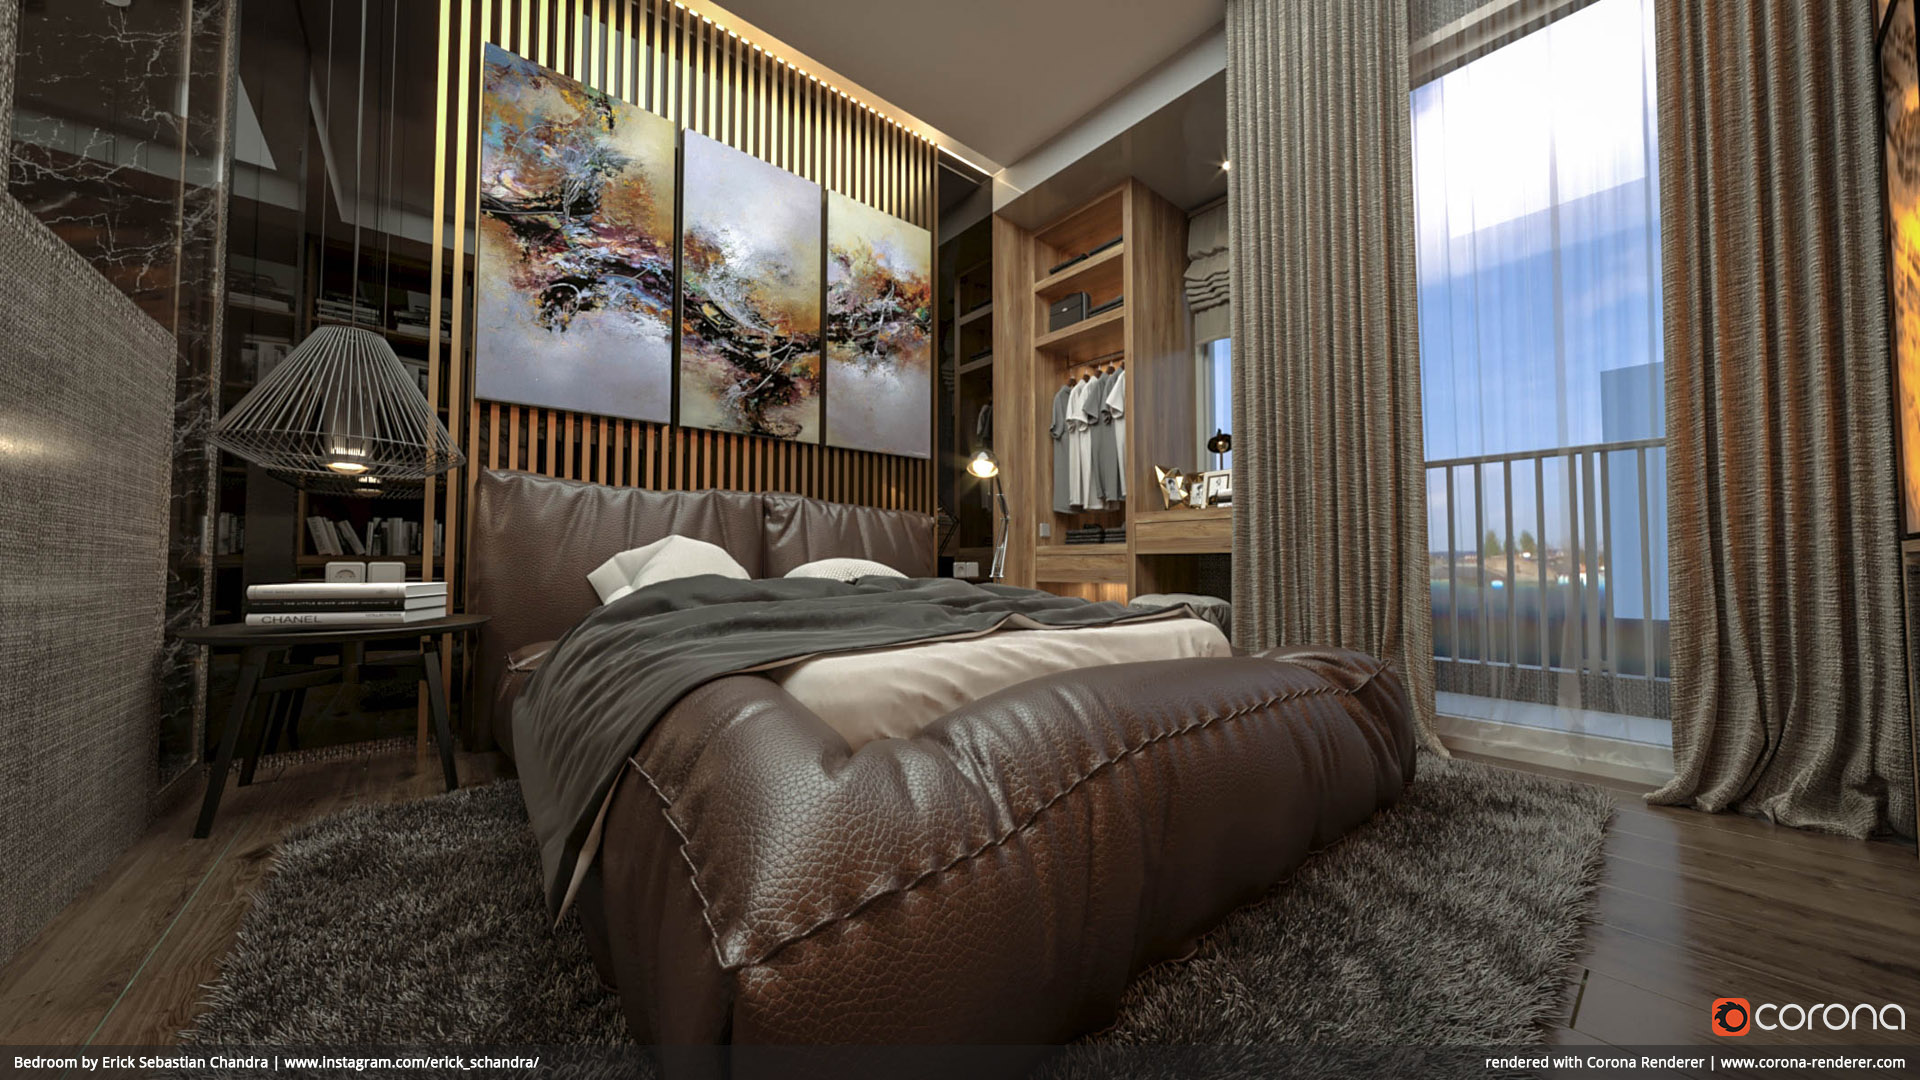
\includegraphics[width=\linewidth]{img/corona_render.jpg}
	\caption{An image generated with the Corona Renderer}
	\label{fig:corona_render}
\end{figure}

The main idea is similar for every renderer:
\begin{enumerate}
	\item A 3D digital scene is described by the objects it contains
	\item A light simulation algorithm runs for every visible pixel from the viewer
	\item Upon object interaction, the shading of the intersected point is computed
	\item When it's done, results in form of a picture ("photograph") called \emph{render} are created
\end{enumerate}

Please see figure ~\ref{fig:path_tracer} for a simple demonstration of this workflow.

\begin{figure}[H]
	\centering
	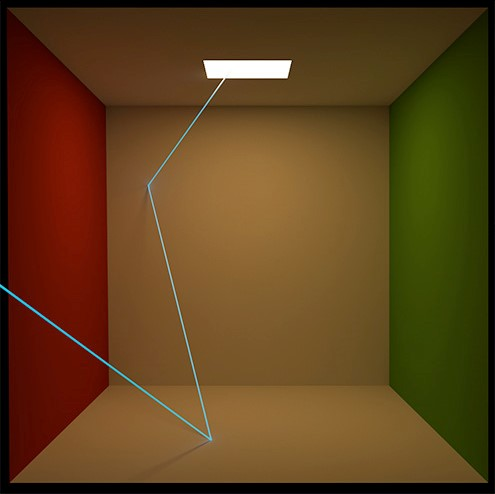
\includegraphics[width=85mm]{img/path_tracer.jpg}
	\caption{A visualization of a light transport algorithm (path tracer)~\cite{mitsubaWeb}}
	\label{fig:path_tracer}
\end{figure}

\subsection{Digital scene}

The basic elements of a digital scene are roughly the same for each renderer. 

\begin{description}
	\item[Camera] A camera in a digital scene works in the same manner as in real life --- it records a picture. Generally, you may define the coordinate position and the viewing vectors but also the properties such as focal distance or the type of film.
	\item[Light source] The scene needs to be illuminated by one or multiple sources in order to be visible. The common kinds of lights are point light, area light, spot light or environment (constant) lighting. 
	\item[Objects] The actual visible content of the scene are objects. Almost all rendering systems offer a choice to either use their precomputed basic geometry such as spheres or triangles or to include a mesh geometry described in an external file (usually created by modeling software). They also have to state their material properties so that the algorithm may correctly interact with them, e.g. diffuse vs. reflective material.
\end{description}

Unfortunately, as each renderer may have a very unique implementation details, the formats of the scenes are vastly different. For example, mitsuba uses XML but PBRT has its own specific format. An example of a simple scene for Mitsuba2 can be found in \ref{fig:example_scene}.

\definecolor{maroon}{rgb}{0.5,0,0}
\definecolor{darkgreen}{rgb}{0,0.5,0}
\lstdefinelanguage{XML}
{
	basicstyle=\ttfamily,
	morestring=[s]{"}{"},
	morecomment=[s]{?}{?},
	morecomment=[s]{!--}{--},
	commentstyle=\color{darkgreen},
	moredelim=[s][\color{black}]{>}{<},
	moredelim=[s][\color{red}]{\ }{=},
	stringstyle=\color{blue},
	identifierstyle=\color{maroon}
}

\begin{figure}[httpb]
\begin{tabular}{p{0.3\textwidth}p{0.6\textwidth}}
\begin{minipage}{0.3\textwidth}
	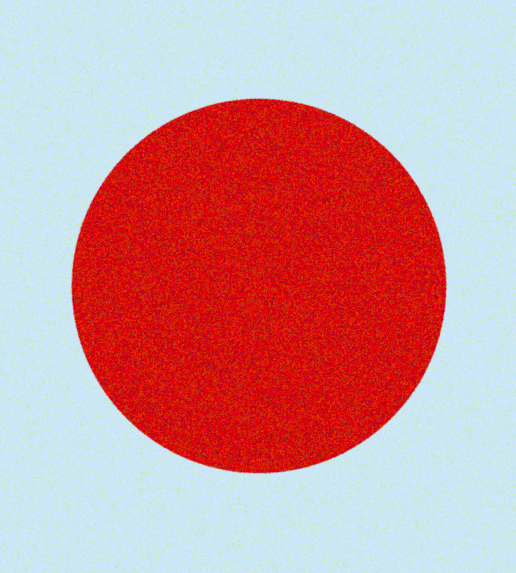
\includegraphics[width=\linewidth]{img/example_scene.png}
\end{minipage}
	&
\begin{minipage}{0.6\textwidth}
	\lstset{language=XML}
	\begin{lstlisting}[basicstyle=\tiny]
<scene version="2.0.0">
 <!-- Light transport algorithm -->
 <integrator type="path"/>
	
 <!-- Camera looking at the sphere -->
 <sensor type="perspective">
  <transform name="to_world">
   <lookat origin="0,-6,0" target="0,0,0" up="0,0,1"/>
  </transform>
 </sensor>
	
 <!-- Red sphere in the middle -->
 <shape type="sphere">
  <bsdf type="diffuse">
   <rgb name="reflectance" value="1.0,0.0,0.0"/>
  </bsdf>
 </shape>
	
 <!-- Light blue light all around the scene-->
 <emitter type="constant">
  <rgb name="radiance" value="0.6,0.8,0.9"/>
 </emitter>
</scene>
	\end{lstlisting}
\end{minipage}
\end{tabular}
\caption{A simple scene rendered with Mitsuba2 (left) along with its scene description (right)}
\label{fig:example_scene}
\end{figure}

\subsection{BRDF}

The fundamental part of the rendering process is its implementation of the light transport simulation. This and the following sections will describe the physics theory and the models behind the light transport. Then we take a look at the specific algorithms. 

The materials of objects inside a scene are described by \emph{Bidirection Distrubtion Reflectance Function}, shortly \emph{BRDF}~\cite{nicodemus1965directional}. It looks as follows:

\begin{equation} \label{eq:brdf}
f_r(\omega_i,\omega_o)=\frac{dL_o(\omega_o)}{L_i(\omega_i)cos\theta_i d\omega_i}
\end{equation}

This function is given the incoming vector $\omega_i$, the outgoing vector $\omega_o$ and it tells us how much radiance is reflected from the direction $\omega_i$ ($L_i(\omega_i)$) to the direction $\omega_o$ ($L_o(\omega_o)$).
An image interpretation of the function is in \ref{fig:brdf}. As it is a distribution function, we can rather describe it as a probability density that a defined amount of light energy gets reflected from $\omega_i$ to $\omega_o$.

\begin{figure}[H]
	\centering
	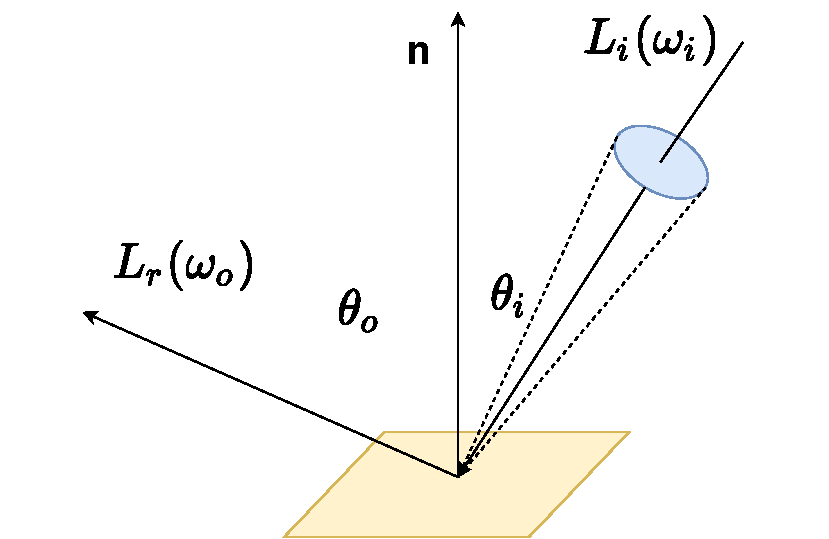
\includegraphics[width=85mm]{img/brdf.pdf}
	\caption{Bidirectional Distribution Reflectance Function}
	\label{fig:brdf}
\end{figure}

In the simplest cases, the BRDF states how reflective the surface of an object is. The renders of diffuse, rough glossy and mirror materials are compared in \ref{fig:compare_brdf}.

\begin{figure}[httpb]
	\begin{tabular}{ccc}
		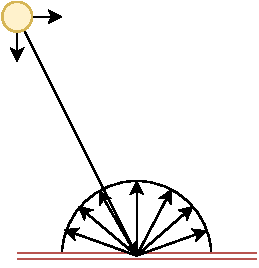
\includegraphics[width=.3\linewidth]{img/brdf_diffuse_diag.pdf}
		&
		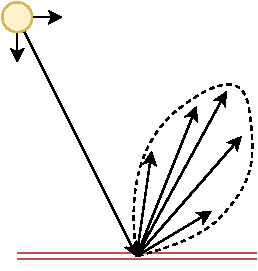
\includegraphics[width=.3\linewidth]{img/brdf_glossy_diag.pdf}
		&
		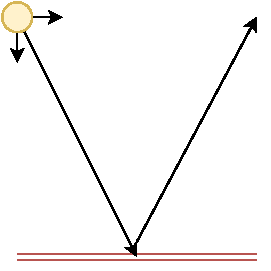
\includegraphics[width=.3\linewidth]{img/brdf_mirror_diag.pdf} \\
		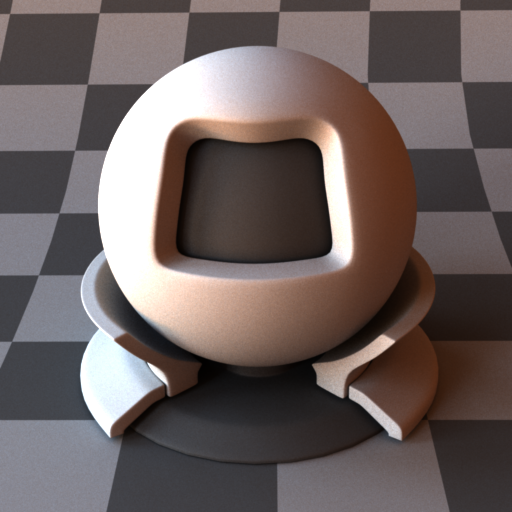
\includegraphics[width=.3\linewidth]{img/brdf_diffuse.png}
		&
		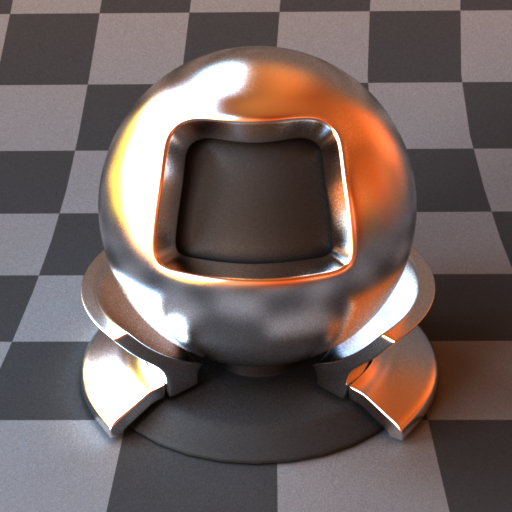
\includegraphics[width=.3\linewidth]{img/brdf_glossy.png}
		&
		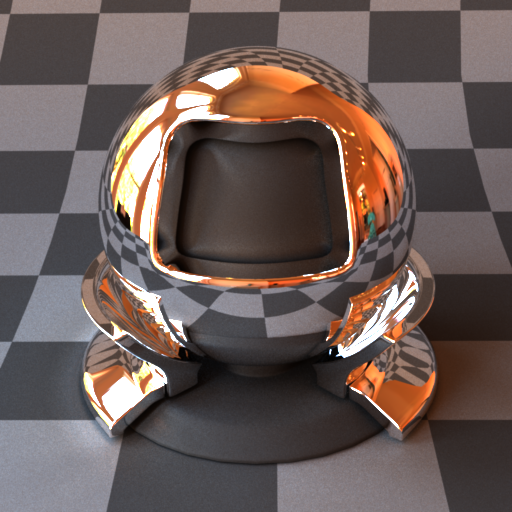
\includegraphics[width=.3\linewidth]{img/brdf_mirror.png}
	\end{tabular}
	\caption{A preview of diffuse (left), glossy (middle) and mirror (right) materials rendered in Mitsuba2 along with their illustrative BRDF visualizations}
	\label{fig:compare_brdf}
\end{figure}


Physically based BRDFs must fulfill several properties~\citealp{duvenhage2013numerical}:
\begin{description}
	\item[Heimholtz reciprocity] The amount of reflected energy from the incoming direction to the outgoing direction is equal to the amount of energy in the reversed directions ($f_r(\omega_i,\omega_o)=f_r(\omega_o,\omega_i)$)
	\item[Energy conservation] The amount of reflected energy cannot be larger than received
	\item[Positivity] BRDF is always positive ($f_r(\omega_i,\omega_o)\le0$)
\end{description}

Note that BRDF concerns only opaque surfaces. There exist multiple distribution functions that describe behavior of other materials, for example:
\begin{description}
	\item[BTDF] Describes light transmission
	\item[BSDF] Combination of BTDF and BRDF (e.g. glass, water)
	\item[BSSRDF] Considers scattering of the light under the surface as well (skin)
\end{description}


\subsection{Global Illumination}

With the BRDF defined, we can now formulate an equation that describes the global illumination of the scene --- illumination of each point from all light sources. It is generally called the \emph{rendering equation}~\cite{kajiya1986rendering}:

\begin{equation}
L_o(x,\omega_o)=L_e(x,\omega_o)+L_r(x,\omega_o)
\end{equation}

Let's break it down first:
\begin{description}
	\item[$x$] is the currently computed point in the scene.
	\item[$L_o$] is the outgoing radiance.
	\item[$L_e$] is the emitted radiance of the point x as x can be on a light source.
	\item[$L_r$] is also called the \emph{reflectance equation} and it states the total amount of the reflected radiance for all the contributions of the incident radiance. Hence, it is an integral over the upper hemisphere over x that look as follows:
	\begin{equation}
	L_r(x,\omega_0)=\int_{\Omega}f_r(x,\omega_o,\omega_i) L_i(x,\omega_,i) cos\theta_i d\omega_i
	\end{equation}
	, where
	\begin{description}
		\item[$f_r(x,\omega_o,\omega_i)$] is the BRDF of x as defined in \ref{eq:brdf}.
		\item[$L_i(x,\omega_i)$] is the incoming radiance from a light source.
	\end{description}
\end{description}

An image interpretation of the reflectance equation can be seen in \ref{fig:refl}.

\begin{figure}[H]
	\centering
	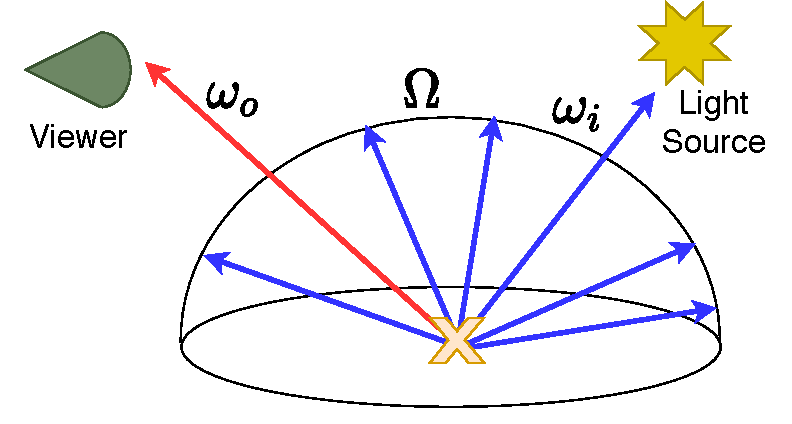
\includegraphics[width=85mm]{img/refl.pdf}
	\caption{Reflectance Equation}
	\label{fig:refl}
\end{figure}

As a matter of fact, each light transport algorithm tries to solve some of the formulations of the rendering equation.

Interestingly, the light transport is recursive in nature. As we can see from the rendering equation, to compute the outgoing radiance at a certain point x, we need to know all the contributed incoming radiances. These do not necessarily have to originate at a light source --- the incoming radiance may come from another non-emitting point y in the scene as a result of the rendering equation computed for the point y.

\subsection{Monte Carlo integration}
Before we proceed to the actual algorithms that evaluate the rendering equation, we briefly introduce a method that is used to approximate the definite integral part of the equation --- \emph{Monte Carlo integration}~\cite{caflisch1998monte}.

Formally, for a multidimensional definite integral
\begin{equation}
I=\int_{\Omega}g(x)dx
\end{equation}
 Monte Carlo (MC) estimates I as 
 \begin{equation}
 \langle I\rangle=\frac{1}{N}\sum_{k=1}^{N}\frac{g(\xi_k)}{p(\xi_k)}; \xi_k\propto p(x)
 \end{equation}

\begin{figure}[H]
	\centering
	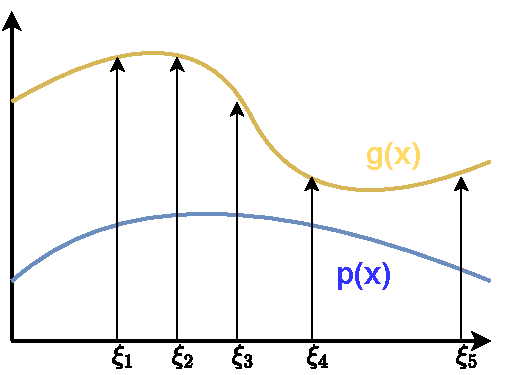
\includegraphics[width=0.5\linewidth]{img/monte_carlo.pdf}
	\caption{Monte Carlo method 2D visualization}
\end{figure}

In other words, Monte Carlo is a non-deterministic method that sums N randomly chosen samples, computes their values and averages them. To reduce variance, an importance sampling is introduced by drawing samples from a distribution $p(x)$ that is chosen for each specific problem to approximate the former $g(x)$ function. This states that if we pick some samples twice as much, we decrease their weight to half.

There exist other methods that are used to approximate integrals such as deterministic quadrature or Markov Chain Monte Carlo (MCMC).

\subsection{Light transport algorithms}

\subsubsection{Path tracing}
There exist various algorithms for the light transport simulation where each has it's own benefits. The one that we will mention the most in this thesis is called the \emph{path tracing}. It's core idea is simple:

\renewcommand{\labelenumii}{\theenumii}
\renewcommand{\theenumii}{\theenumi.\arabic{enumii}.}
\begin{enumerate}
	\item Shoot a primary ray $r$ from camera for each pixel in the image plane into the scene.
	\item If $r$ hits a non-emitting object at point $x$:
	\begin{enumerate}
		\item Compute BRDF at $x$.
		\item Generate a new random direction $\omega$. Ideally, the distribution of the generated direction should be proportional to the BRDF --- e.g. diffuse BRDF would generate a direction  uniformly over a hemisphere while glossy BRDF would prioritize samples from the reflectance lobe (look at \ref{fig:compare_brdf}).
		\item Add the BRDF value to the final color of the pixel.
		\item Check for a terminating condition --- there exist several options, usually a combination of them is:
			\begin{description}
				\item [Maximum depth] User specified maximum number of recursion.
				\item [Russian Roulette] Randomly choose if the ray survives, with each ray the chance lowers.
				\item [BRDF-proportional] Depending on the surface material, we decide whether the ray survives or not. For example, reflective or refractive surface need a lot more samples than diffuse surfaces.
			\end{description}
		\item In case the termination was not successful, bounce -- shot a secondary ray $r$ from point $x$ in the direction $\omega$ and continue from step 2.
	\end{enumerate}
	\item If $r$ hits an emitting object (light source), add it's emission $L_e$ to the final color of the pixel
	\item If it no scene geometry is hit, terminate the algorithm. In case this is the primary ray, the pixel is the color of a surrounding light.
\end{enumerate}

The bouncing of the light in the scene nicely correlates with the recursive nature of the rendering equation. Even though the path tracing is a slow algorithm (e.g. not suitable for real-time rendering in games), it's variations can be extremely accurate, even indistinguishable from a real photograph. 


\paragraph{MIS}

In the algorithm described above, the direct illumination computation is dependent only on the BRDF of each intersected point and consequent walk to the light source. However, such scenario that the light source is hit at the end of every walk is greatly dependent on the number of samples and the maximum allowed depth of the recursion. Consequently, this creates variance which can be easily improved the integration of the \emph{multiple importance sampling} (MIS). This involves a combination of the BRDF proportional sampling and the light source sampling --- in each step of the path tracing, every light source that is visible from the intersected point contributes to it's value. Both sampling methods are, of course, weighted to avoid an over-illumination. 

\paragraph{Volumes}

Another aspect that needs to be accounted for in the rendering process generally are volumetric objects such as fogs or smokes. Generally, there are two ways that a volumetric object may effect the light passing through. Is is either attenuating the light by absorbing it or scattering to different directions. Or it can also strengthen it by emitting light (e.g. flame) or scattering light from different directions to the current one.

A single walk of a path tracer capable of volume tracing and MIS sampling is visualized in \ref{fig:path_tracer_vis}.

\renewcommand\thesubfigure{\arabic{subfigure}}
\begin{figure}
	\begin{tabular}{cc}
		\begin{subfigure}
			{0.45\textwidth}\centering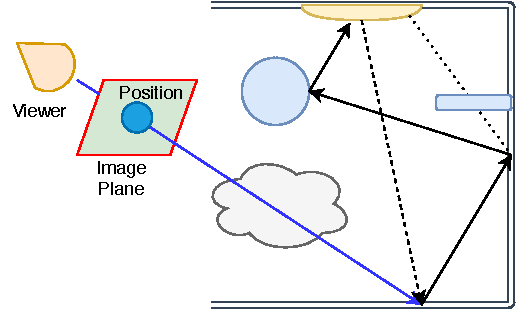
\includegraphics[width=\linewidth]{img/path_tracer_step1.pdf}
			\caption{Ray at pixel on image plane created (from blue dot along blue line)}
		\end{subfigure}
		&
		\begin{subfigure}
			{0.45\textwidth}\centering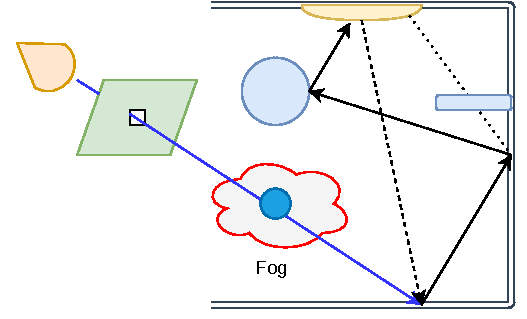
\includegraphics[width=\linewidth]{img/path_tracer_step2.pdf}
			\caption{Passing volume, attenuation}
		\end{subfigure} \\
		\begin{subfigure}
			{0.45\textwidth}\centering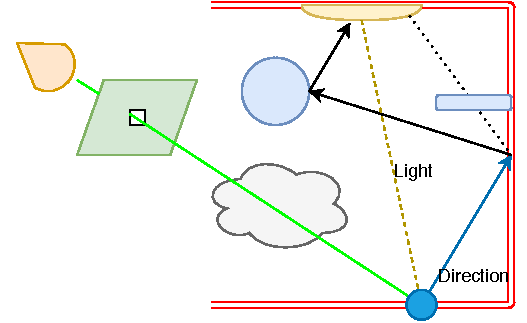
\includegraphics[width=\linewidth]{img/path_tracer_step3.pdf}
			\caption{ Geometry hit,  generate new direction, compute BRDF + light contribution}
		\end{subfigure} 
		&
		\begin{subfigure}
			{0.45\textwidth}\centering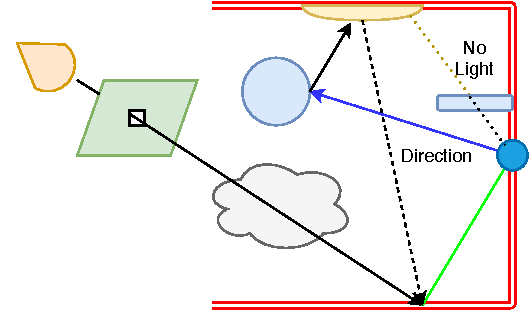
\includegraphics[width=\linewidth]{img/path_tracer_step4.pdf}
			\caption{Geometry hit, generate new direction, compute BRDF (no light - obscured)}
		\end{subfigure} \\
		\multicolumn{2}{c}{		
		\begin{subfigure}
				{0.45\textwidth}\centering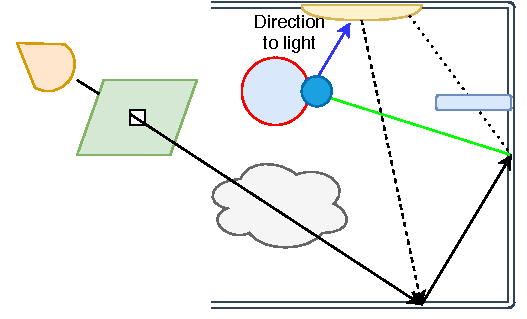
\includegraphics[width=\linewidth]{img/path_tracer_step5.pdf}
				\caption{Geometry hit, generate new direction - points to light, add contribution and terminate}
		\end{subfigure}}
	\end{tabular}
	\caption{A visualization of a single walk in path tracer}
	\label{fig:path_tracer_vis}
\end{figure}


\subsubsection{Other methods}
There exist other techniques and variations for the global illumination rendering. We mention some of them only briefly as the path tracing is of our main concern in this thesis due to its physically based and unbiased properties:

\begin{description}
	\item[Ray tracing]\cite{glassner1989introduction} Similar to path tracing but there are no bounces from surfaces, simulates only reflections, refractions, scattering etc. Capable of realtime rendering these days.
	\item[Photon mapping]\cite{jensen2001realistic} Two rays are traced independently --- from camera and from a light source until termination, then the radiance is computed based in their final positions. Faster at some scenarios but biased (does not have to converge to a correct solution).
	\item[Radiosity]\cite{sillion1994radiosity}Uses finite element method instead of Monte Carlo. View independent, light is traced from the source and bounced (possibly) to the viewer. Good for precomputations. 
\end{description}


